% !TEX root = ../main.tex
\chapter{Marc teòric i contextualització}
\label{chap:marc_teoric}

Aquest capítol estableix els fonaments per a la comprensió i la lectura crítica de la comparació d'agents. En primer lloc, es descriu el domini del combat Pokémon, les seves mecàniques de combat i el format \texttt{gen9randombattle}. En segon lloc, es formalitza el problema des de la teoria de jocs i la presa de decisions sota incertesa (POMDP i POSG). En tercer lloc, es revisa l'estat de l'art en IA aplicada a jocs complexos i específicament a Pokémon. Finalment, es presenten els fonaments teòrics dels cinc paradigmes d'agents estudiats.

% ============================================================
\section{Pokémon com a domini de decisió}
\label{sec:pokemon_joc}

Abans de formalitzar el problema des del punt de vista de la Teoria de Jocs i dels processos de decisió sota incertesa, cal contextualitzar el domini real del combat Pokémon. El càlcul d'estadístiques, la matriu de tipus, la velocitat, les condicions d'estat i les fonts d'estocasticitat conformen el marc mecànic sobre el qual els agents d'intel·ligència artificial han d'avaluar l'estat del joc i executar les seves estratègies.

\subsection{Què és Pokémon i com es desenvolupa una batalla}

\textit{Pokémon} és una franquícia de videojocs creada l'any 1996 per Satoshi Tajiri i la companyia Game Freak per a la consola Game Boy de Nintendo~\cite{pokemon_official}. El nom \textbf{Pokémon} prové de la contracció de la denominació anglesa \textbf{\emph{Pocket Monsters}} (\emph{Poketto Monstā} en japonès), fent referència a les criatures que es capturen en esferes portàtils (Poké Balls), es col·leccionen, s'entrenen i participen en combats. Coincidint amb la celebració del seu \textbf{30è aniversari (1996--2026)}, la franquícia s'ha convertit en un fenomen cultural global que abasta videojocs, sèries d'animació, cartes col·leccionables (TCG) i entreteniment multimèdia, on l'estratègia de combat manté un paper central en l'àmbit competitiu.

\begin{figure}[htbp]
    \centering
    
\includegraphics[width=0.25\linewidth]{images/logos/pokemon30.png}
    \caption{Logotip commemoratiu del 30è aniversari de la franquícia Pokémon (1996--2026), que celebra tres dècades d'història i d'impacte cultural global en l'entreteniment multimèdia i els videojocs.}
    \label{fig:pokemon_30_logo}
\end{figure}

En una batalla individual (\textit{Singles}), cada jugador disposa habitualment d'un equip de sis Pokémon, però només un és actiu a cada banda. L'objectiu és debilitar tots els membres de l'equip rival abans que el rival faci el mateix.

En cada torn, un jugador pot escollir un dels moviments disponibles o canviar el Pokémon actiu per un membre no debilitat de l'equip. Un Pokémon pot conèixer com a màxim quatre moviments. Alguns causen dany; d'altres modifiquen estadístiques, imposen una condició d'estat, alteren el camp o permeten canviar conservant la iniciativa. Els dos jugadors envien l'acció sense conèixer la decisió actual de l'altre. El motor ordena les accions segons la prioritat i la velocitat, comprova la precisió i resol el dany i els efectes secundaris.

Aquesta estructura fa que una acció no es pugui valorar de manera aïllada. Un atac molt potent pot ser inútil contra una immunitat de tipus; un canvi pot evitar un debilitament, però permetre que el rival col·loqui un perill d'entrada (\emph{hazards}); i un moviment de preparació (\emph{setup}) pot sacrificar el torn actual per augmentar la probabilitat de guanyar els següents.

Aquesta explicació inicial ofereix una introducció general i conceptual a la dinàmica de la batalla. En les subseccions següents es desenvolupen amb més profunditat i detall cadascun dels seus components mecànics fonamentals: la formulació de les estadístiques de combat, la matriu d'efectivitat de tipus, les regles de velocitat i prioritat, les condicions d'estat i les fonts d'estocasticitat.

\begin{figure}[htbp]
    \centering
    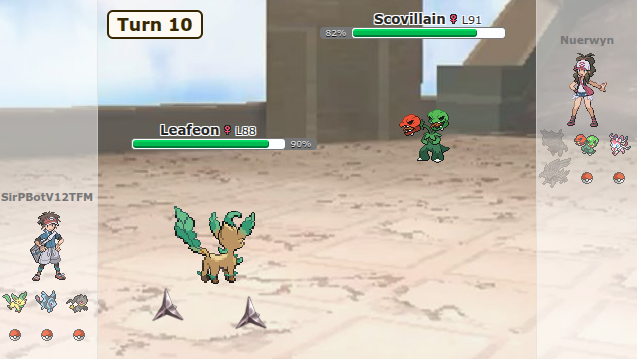
\includegraphics[width=0.88\linewidth]{images/diagrams/battle_pkmn_shwd.png}
    \caption{Captura de la interfície de Pokémon Showdown durant un combat, on s'observen els Pokémon actius de cada bàndol, les banquetes de substituts (actius, debilitats o ocults), els nivells, percentatges de vida (HP) i la informació visible de la batalla.}
    \label{fig:pokemon_showdown_battle}
\end{figure}

\subsection{De l'espècie a les estadístiques finals}
\label{subsec:stats}

Cada Pokémon pertany a una espècie concreta amb atributs únics i disposa de sis estadístiques de combat: punts de salut (\textit{Hit Points}, HP), atac, defensa, atac especial, defensa especial i velocitat~\cite{bulbapedia_pokemon,bulbapedia_stats}. Els HP determinen quant dany pot rebre; atac i defensa intervenen en els moviments físics; atac especial i defensa especial, en els moviments especials; i la velocitat decideix quin Pokémon actua abans.

La xifra final que mostra el joc es construeix a partir de cinc components:
\begin{enumerate}
    \item \textbf{Estadística base ($B$).} Pròpia de l'espècie. Dos Pikachu comparteixen les mateixes estadístiques base, però no necessàriament les mateixes xifres finals.
    \item \textbf{Nivell ($L$).} Escala el valor final. Random Battle utilitza el nivell com a mecanisme d'equilibri entre espècies.
    \item \textbf{Valors individuals (IV).} Cada estadística té un IV enter entre 0 i 31~\cite{bulbapedia_iv}.
    \item \textbf{Punts d'esforç (EV).} Es poden distribuir fins a 510 EV en total, amb un màxim efectiu de 252 en una mateixa estadística~\cite{bulbapedia_ev}.
    \item \textbf{Naturalesa ($N$).} La majoria de naturaleses multipliquen una estadística per 1,1 i una altra per 0,9~\cite{bulbapedia_nature}.
\end{enumerate}

Per a qualsevol estadística de combat diferent dels HP (Atac, Defensa, Atac Especial, Defensa Especial i Velocitat), la fórmula general d'escalat és:

\vspace{16pt}
{\large
    \begin{equation}
        \mathrm{Stat} =
        \left\lfloor
        \left(
        \left\lfloor
        \frac{(2B+\mathrm{IV}+\lfloor \mathrm{EV}/4\rfloor)L}{100}
        \right\rfloor + 5
        \right)N
        \right\rfloor .
        \label{eq:stat_formula}
    \end{equation}
}
\vspace{16pt}

Per contra, els punts de salut (HP) segueixen un càlcul diferent per dues raons mecàniques: en primer lloc, cap naturalesa modifica els HP (no s'aplica el multiplicador $N$); en segon lloc, s'afegeix el terme $+L + 10$ en comptes de la constant fixa $+5$ per tal que la salut màxima escali de manera proporcional al nivell $L$ de la criatura. Excepte casos especials com Shedinja (els HP del qual estan fixats permanentment pel motor de joc en $1$ HP independentment del nivell, IVs o EVs), la fórmula de càlcul dels HP és:

\vspace{16pt}
{\large
    \begin{equation}
        \mathrm{HP} =
        \left\lfloor
        \frac{(2B+\mathrm{IV}+\lfloor \mathrm{EV}/4\rfloor)L}{100}
        \right\rfloor + L + 10 .
        \label{eq:hp_formula}
    \end{equation}
}
\vspace{16pt}
\begin{table}[htbp]
\centering
\caption{Exemple numèric de la fórmula~\eqref{eq:stat_formula}--\eqref{eq:hp_formula} per a Pikachu a nivell 100. Les bases són les de l'espècie~\cite{bulbapedia_stats}; IV, EV i naturalesa Timid (velocitat $\times 1{,}1$, atac $\times 0{,}9$) són una configuració il·lustrativa, no un set de Random Battle.}
\label{tab:pikachu_stat_example}
\small
\begin{tabular}{lrrrrr}
\toprule
\textbf{Estadística} & \textbf{Base $B$} & \textbf{IV} & \textbf{EV} & \textbf{$N$} & \textbf{Valor final} \\
\midrule
HP & 35 & 31 & 0 & --- & 211 \\
Atac & 55 & 31 & 0 & $0{,}9$ & 131 \\
Defensa & 40 & 31 & 0 & $1{,}0$ & 116 \\
Atac especial & 50 & 31 & 0 & $1{,}0$ & 136 \\
Defensa especial & 50 & 31 & 0 & $1{,}0$ & 136 \\
Velocitat & 90 & 31 & 252 & $1{,}1$ & 306 \\
\bottomrule
\end{tabular}
\end{table}

\vspace{12pt}

Com s'observa a la Taula~\ref{tab:pikachu_stat_example}, les xifres finals calculades determinen el perfil competitiu real de la criatura durant el combat. Aquestes estadístiques finals ---especialment la Velocitat efectiva ($306$) i la salut màxima ($\mathrm{HP}=211$)--- són els valors concrets que el motor de Pokémon Showdown utilitza a cada torn per determinar l'ordre d'actuació i l'abast del dany produït. Conseqüentment, aquests valors constitueixen la base d'informació sobre la qual els agents d'IA estimen la velocitat relativa, el dany sota tirada i el risc de debilitament.

\subsection{Tipus elementals, matriu d'efectivitat i categories de moviment}
\label{subsec:tipus}

Un dels pilars estratègics del combat Pokémon és la relació elemental entre els 18 tipus existents (Foc, Aigua, Planta, etc.). Cal distingir clarament entre el \textbf{tipus del Pokémon} i el \textbf{tipus del moviment}:
\begin{itemize}
    \item \textbf{Tipus del Pokémon (funció defensiva):} Cada criatura disposa d'un o dos tipus elementals pròpis (tipus únic o \textbf{doble tipus}) que determinen les febleses, resistències i immunitats quan \emph{rep} un atac rival.
    \item \textbf{Tipus del moviment (funció ofensiva):} Atribut propi de l'acció executada. Un Pokémon no està restringit a utilitzar atacs del seu mateix tipus elemental (p. ex., un Pokémon de Foc pot llançar un atac de Terra). Tanmateix, quan el tipus del moviment coincideix amb un dels seus tipus pròpis, el joc atorga una bonificació extra del $+50\%$ al dany denominada \textbf{STAB} (\emph{Same Type Attack Bonus}, multiplicador $\times 1{,}5$).
\end{itemize}

Quan un Pokémon té \textbf{doble tipus}, els multiplicadors de la matriu d'efectivitat (Taula~\ref{tab:type_chart}) es combinen multiplicativament ($M = M_1 \times M_2$), generant efectes de \textbf{debilitat doble} ($\times 4$, p. ex., Roca contra Foc/Volador: $2 \times 2 = 4$), \textbf{resistència doble} ($\times 0{,}25$, p. ex., Planta contra Acer/Volador), \textbf{neutralització} ($\times 1$, p. ex., Lluita contra Insecte/Roca: $2 \times 0{,}5 = 1$) o \textbf{immunitat absoluta} ($\times 0$, p. ex., Elèctric contra Aigua/Terra: $2 \times 0 = 0$).

Els moviments es classifiquen en tres categories principals:
\begin{enumerate}
    \item \textbf{Físics (Atac vs. Defensa):} Atacs de contacte físic o força directa.
    \item \textbf{Especials (Atac Esp. vs. Def. Esp.):} Atacs d'energia, distància o projectils elementals.
    \item \textbf{D'estat / Suport:} No causen dany directe; s'utilitzen per induir \textbf{condicions d'estat primàries} (com cremada, paràlisi o verí; vegeu Secció~\ref{subsec:status}), modificar estadístiques, alterar el clima o col·locar perills d'entrada com \emph{Stealth Rock}.
\end{enumerate}

La diferenciació entre la via física i especial és crucial: la majoria de Pokémon s'especialitzen en un perfil defensiu físic o especial concret, la qual cosa obliga els agents d'IA a avaluar la categoria d'atac que exploti la feblesa estructural del rival.

% Taula de Tipus de Pokémon — Matriu 18×18 de multiplicadors de dany
% Fila = Tipus de l'atac, Columna = Tipus del defensor
% Requereix: \usepackage[table]{xcolor}, \usepackage{booktabs}, \usepackage{textcomp}

% Definició de colors per tipus
\definecolor{typNormal}{HTML}{A8A878}
\definecolor{typFoc}{HTML}{F08030}
\definecolor{typAigua}{HTML}{6890F0}
\definecolor{typPlanta}{HTML}{78C850}
\definecolor{typElectric}{HTML}{F8D030}
\definecolor{typGel}{HTML}{98D8D8}
\definecolor{typLluita}{HTML}{C03028}
\definecolor{typVeri}{HTML}{A040A0}
\definecolor{typTerra}{HTML}{E0C068}
\definecolor{typVolador}{HTML}{A890F0}
\definecolor{typPsiquic}{HTML}{F85888}
\definecolor{typInsecte}{HTML}{A8B820}
\definecolor{typRoca}{HTML}{B8A038}
\definecolor{typFantasma}{HTML}{705898}
\definecolor{typDrac}{HTML}{7038F8}
\definecolor{typFosc}{HTML}{705848}
\definecolor{typAcer}{HTML}{B8B8D0}
\definecolor{typFada}{HTML}{EE99AC}

% Comandes per cel·les d'efectivitat
\newcommand{\SE}{\cellcolor{green!40}\textbf{2}}
\newcommand{\NV}{\cellcolor{red!20}{\textonehalf}}
\newcommand{\IM}{\cellcolor{gray!70}\textcolor{white}{\textbf{0}}}
\newcommand{\NE}{}

% Comanda per capçaleres de tipus amb color
\newcommand{\ty}[2]{\cellcolor{#1}\textcolor{white}{\textbf{#2}}}

\begin{table}[H]
\centering
\caption{Matriu de la Taula de Tipus (Gen.\ VI--IX). Files = tipus de l'atac, columnes = tipus del defensor. \colorbox{green!40}{\scriptsize\textbf{2}} = Super Effective ($\times 2$), \colorbox{red!20}{\scriptsize\textonehalf} = Not Very Effective ($\times 0.5$), \colorbox{gray!70}{\scriptsize\textcolor{white}{\textbf{0}}} = Immunitat ($\times 0$), buit = Neutral ($\times 1$).}
\label{tab:type_chart}
\vspace{2pt}
\begin{adjustbox}{max width=\textwidth}
\tiny
\setlength{\tabcolsep}{2.5pt}
\renewcommand{\arraystretch}{1.2}
\begin{tabular}{>{\bfseries}l|c|c|c|c|c|c|c|c|c|c|c|c|c|c|c|c|c|c|}
\cline{2-19}
& \ty{typNormal}{NOR} & \ty{typFoc}{FOC} & \ty{typAigua}{AIG} & \ty{typPlanta}{PLA} & \ty{typElectric}{ELE} & \ty{typGel}{GEL} & \ty{typLluita}{LLU} & \ty{typVeri}{VER} & \ty{typTerra}{TER} & \ty{typVolador}{VOL} & \ty{typPsiquic}{PSI} & \ty{typInsecte}{INS} & \ty{typRoca}{ROC} & \ty{typFantasma}{FAN} & \ty{typDrac}{DRA} & \ty{typFosc}{FOS} & \ty{typAcer}{ACE} & \ty{typFada}{FAD} \\
\hline
\ty{typNormal}{NOR}   & \NE & \NE & \NE & \NE & \NE & \NE & \NE & \NE & \NE & \NE & \NE & \NE & \NV & \IM & \NE & \NE & \NV & \NE \\ \hline
\ty{typFoc}{FOC}      & \NE & \NV & \NV & \SE & \NE & \SE & \NE & \NE & \NE & \NE & \NE & \SE & \NV & \NE & \NV & \NE & \SE & \NE \\ \hline
\ty{typAigua}{AIG}    & \NE & \SE & \NV & \NV & \NE & \NE & \NE & \NE & \SE & \NE & \NE & \NE & \SE & \NE & \NV & \NE & \NE & \NE \\ \hline
\ty{typPlanta}{PLA}   & \NE & \NV & \SE & \NV & \NE & \NE & \NE & \NV & \SE & \NV & \NE & \NV & \SE & \NE & \NV & \NE & \NV & \NE \\ \hline
\ty{typElectric}{ELE} & \NE & \NE & \SE & \NV & \NV & \NE & \NE & \NE & \IM & \SE & \NE & \NE & \NE & \NE & \NV & \NE & \NE & \NE \\ \hline
\ty{typGel}{GEL}      & \NE & \NV & \NV & \SE & \NE & \NV & \NE & \NE & \SE & \SE & \NE & \NE & \NE & \NE & \SE & \NE & \NV & \NE \\ \hline
\ty{typLluita}{LLU}   & \SE & \NE & \NE & \NE & \NE & \SE & \NE & \NV & \NE & \NV & \NV & \NV & \SE & \IM & \NE & \SE & \SE & \NV \\ \hline
\ty{typVeri}{VER}     & \NE & \NE & \NE & \SE & \NE & \NE & \NE & \NV & \NV & \NE & \NE & \NE & \NV & \NV & \NE & \NE & \IM & \SE \\ \hline
\ty{typTerra}{TER}    & \NE & \SE & \NE & \NV & \SE & \NE & \NE & \SE & \NE & \IM & \NE & \NV & \SE & \NE & \NE & \NE & \SE & \NE \\ \hline
\ty{typVolador}{VOL}  & \NE & \NE & \NE & \SE & \NV & \NE & \SE & \NE & \NE & \NE & \NE & \SE & \NV & \NE & \NE & \NE & \NV & \NE \\ \hline
\ty{typPsiquic}{PSI}  & \NE & \NE & \NE & \NE & \NE & \NE & \SE & \SE & \NE & \NE & \NV & \NE & \NE & \NE & \NE & \IM & \NV & \NE \\ \hline
\ty{typInsecte}{INS}  & \NE & \NV & \NE & \SE & \NE & \NE & \NV & \NV & \NE & \NV & \SE & \NE & \NE & \NV & \NE & \SE & \NV & \NV \\ \hline
\ty{typRoca}{ROC}     & \NE & \SE & \NE & \NE & \NE & \SE & \NV & \NE & \NV & \SE & \NE & \SE & \NE & \NE & \NE & \NE & \NV & \NE \\ \hline
\ty{typFantasma}{FAN} & \IM & \NE & \NE & \NE & \NE & \NE & \NE & \NE & \NE & \NE & \SE & \NE & \NE & \SE & \NE & \NV & \NE & \NE \\ \hline
\ty{typDrac}{DRA}     & \NE & \NE & \NE & \NE & \NE & \NE & \NE & \NE & \NE & \NE & \NE & \NE & \NE & \NE & \SE & \NE & \NV & \IM \\ \hline
\ty{typFosc}{FOS}     & \NE & \NE & \NE & \NE & \NE & \NE & \NV & \NE & \NE & \NE & \SE & \NE & \NE & \SE & \NE & \NV & \NE & \NV \\ \hline
\ty{typAcer}{ACE}     & \NE & \NV & \NV & \NE & \NV & \SE & \NE & \NE & \NE & \NE & \NE & \NE & \SE & \NE & \NE & \NE & \NV & \SE \\ \hline
\ty{typFada}{FAD}     & \NE & \NV & \NE & \NE & \NE & \NE & \SE & \NV & \NE & \NE & \NE & \NE & \NE & \NE & \SE & \SE & \NV & \NE \\ \hline
\end{tabular}
\end{adjustbox}
\end{table}


\subsection{Teracristal·lització (Generació~IX)}
\label{subsec:teracristallitzacio}

La \textbf{Teracristal·lització} (\emph{Terastallization} o \emph{Tera}) és la mecànica transformativa exclusiva de la novena generació (\emph{Pokémon Scarlet \& Violet}, 2022) utilitzada en el format \texttt{gen9randombattle}~\cite{bulbapedia_terastal}. Aquesta mecànica permet a cada jugador transformar un dels seus Pokémon una sola vegada per combat, canviant els seus tipus elementals originals per un únic \textbf{Tipus Tera} (\emph{Tera Type}) seleccionat d'entre els 18 tipus de la matriu d'efectivitat (Taula~\ref{tab:type_chart}).

La Teracristal·lització altera la dinàmica del combat a dos nivells clau:
\begin{itemize}
    \item \textbf{Nivell defensiu:} El Pokémon adopta immediatament el Tipus Tera com a únic tipus defensiu actiu, substituint completament les seves febleses i resistències d'origen. Per exemple, un Pokémon de tipus Aigua/Volador que teracristal·litza a tipus Planta passa a ser defensivament de tipus Planta pur, convertint una feblesa fatal de $4\times$ a l'Electricitat en una resistència del $0{,}5\times$.
    \item \textbf{Nivell ofensiu (STAB millorat):} Els atacs del nou Tipus Tera obtenen la bonificació de STAB ($1{,}5\times$). Tanmateix, si el Tipus Tera coincideix amb un dels tipus originals de la criatura (p. ex., un Pokémon de Foc teracristal·litzant a Foc), la bonificació de STAB s'amplifica fins al \textbf{$2{,}0\times$} ($+100\%$ de dany). A més, el Pokémon conserva la bonificació de STAB $1{,}5\times$ en els atacs dels seus tipus primaris d'origen.
\end{itemize}

Des de la perspectiva de la presa de decisions en IA, la Teracristal·lització és un recurs d'ús únic d'alta rellevància estratègica. Permet realitzar accions de canvi de tipus instantani (\emph{type-shift}) per sobreviure a atacs directes, anular un atac supereficaç del rival i capgirar l'estat del combat en un únic torn, constituint un dels punts d'avaluació més complexos per a les polítiques de decisió dels agents.

\subsection{Velocitat, prioritat i l'empat de velocitat}
\label{subsec:velocitat}

La \textbf{Velocitat} és una de les estadístiques més determinants en el combat Pokémon competitiu. Atacar primer no només concedeix la iniciativa tàctica (\emph{tempo}), sinó que atorga la capacitat de debilitar la criatura rival abans que aquesta pugui executar la seva acció en aquell torn, anul·lant per complet el seu potencial de dany. Conseqüentment, saber quin Pokémon actuarà abans és un càlcul fonamental per als agents d'IA en avaluar els riscos i les oportunitats de cada moviment.

En cada torn, el motor de joc ordena l'execució de les accions seguint dos criteris seqüencials:

\begin{enumerate}
    \item \textbf{Prioritat del moviment:} Cada moviment té un valor de prioritat discret que varia entre $+5$ i $-7$. Els moviments de prioritat alta, com \emph{Protect} ($+4$), \emph{Extreme Speed} ($+2$) o \emph{Quick Attack} ($+1$), s'executen sempre abans que qualsevol moviment de prioritat neutra ($0$), independentment de la Velocitat dels Pokémon. Per contra, moviments d'alta utilitat tàctica com \emph{Trick Room} ($-7$) s'executen al final del torn.
    \item \textbf{Velocitat efectiva:} Si dos moviments tenen la mateixa prioritat (habitualment $0$), actua primer el Pokémon que tingui una Velocitat efectiva més alta en aquell torn, tenint en compte l'estadística final, els canvis d'etapa (de $-6$ a $+6$), els objectes equipats (com \emph{Choice Scarf}, que augmenta la velocitat en un $50\%$) i les condicions d'estat (la paràlisi redueix la velocitat a la meitat).
\end{enumerate}

Quan dos Pokémon tenen exactament la mateixa prioritat i la mateixa Velocitat efectiva final, es produeix un \textbf{empat de velocitat} (\emph{Speed Tie}). El motor de joc resol aquest empat mitjançant una decisió aleatòria al $50\%$ ($p=0{,}5$).

\subsection{Condicions d'estat primàries}
\label{subsec:status}

Com s'ha introduït en les categories de moviment (Secció~\ref{subsec:tipus}), els moviments d'estat o suport (com \emph{Will-O-Wisp} o \emph{Thunder Wave}) i certs efectes secundaris d'atacs físics o especials tenen la capacitat d'imposar \textbf{condicions d'estat primàries}. Aquestes alteracions són persistents i afecten negativament les capacitats operatives d'un Pokémon. Un Pokémon només pot patir una condició d'estat primària de manera simultània. A la Taula~\ref{tab:status} es resumeixen les principals condicions d'estat i els seus efectes mecànics en el combat.

\begin{table}[htbp]
    \centering
    \small
    \caption{Condicions d'estat primàries principals i els seus efectes mecànics en el combat Pokémon.}
    \label{tab:status}
    \vspace{2pt}
    \begin{tabular}{llp{7.5cm}}
        \toprule
        \textbf{Estat} & \textbf{Efecte en combat}               & \textbf{Mecànica i impacte tàctic}                                                                           \\ \midrule
        Cremada        & $\downarrow 50\%$ Atac físic            & Causa un dany recurrent d'1/16 dels HP màxims per torn i redueix a la meitat l'Atac físic efectiu.           \\
        Paràlisi       & $\downarrow 50\%$ Velocitat (Gen. VII+) & Redueix la Velocitat a la meitat i introdueix un $25\%$ de probabilitat de no actuar per torn.               \\
        Verí / Tòxic   & Dany recurrent per torn                 & El verí estàndard treu 1/8 dels HP per torn; el verí tòxic incrementa el dany a cada torn ($1/16, 2/16...$). \\
        Son            & Inhabilitació temporal                  & El Pokémon no pot actuar durant 1--3 torns consecutius.                                                      \\
        Congelació     & Inhabilitació estocàstica               & El Pokémon no pot actuar; té un $20\%$ de probabilitat de descongelar-se a cada torn.                        \\ \bottomrule
    \end{tabular}
\end{table}

Des de la perspectiva de la presa de decisions, induir una condició d'estat pot ser estratègicament superior a causar dany immediat. Per exemple, cremar un atacant físic enreda irreversiblement el seu potencial ofensiu, mentre que paralitzar un Pokémon ràpid permet a l'agent recuperar la iniciativa de velocitat en el combat.

\subsection{Fonts d'estocasticitat irreductibles}
\label{subsec:estocasticitat}

El combat Pokémon és un entorn fortament estocàstic. Fins i tot quan un agent disposa d'informació completa sobre l'estat actiu, el resultat d'una decisió està subjecte a tres fonts d'aleatorietat irreductibles administrades pel simulador de joc~\cite{smogon_damage,smogon_metagame,bulbapedia_stats}:

\begin{enumerate}
    \item \textbf{Tirada de dany (\emph{Damage Roll}):} El dany calculat per les fórmules oficials no és un valor fix, sinó que es multiplica per un factor aleatori extret d'una distribució uniforme discreta de 16 valors entre $0{,}85$ i $1{,}00$ ($\{0{,}85, 0{,}86, \dots, 1{,}00\}$)~\cite{smogon_damage}. Així, un mateix atac pot debilitar un rival si es dona una tirada alta ($1{,}00$), però deixar-lo amb vida si la tirada és baixa ($0{,}85$).
    \item \textbf{Precisió i evasió (\emph{Accuracy}):} Molts moviments potents no tenen una precisió del $100\%$ (p. ex., \emph{Hydro Pump} amb $80\%$ o \emph{Focus Blast} amb $70\%$)~\cite{bulbapedia_stats}. L'agent ha de ponderar el dany esperat davant del risc de fallar l'atac i regalar un torn d'iniciativa al rival.
    \item \textbf{Cop crític (\emph{Critical Hit}):} A la Generació~IX, la probabilitat base que un atac sigui crític és d'1 de cada 24 vegades ($p_{\mathrm{crit}} \approx 4{,}17\%$)~\cite{bulbapedia_stats,smogon_damage}. Un cop crític aplica un multiplicador de $\times 1{,}5$ al dany, ignora els augments defensius del rival i ignora les reduccions d'atac de l'usuari.
\end{enumerate}

Matemàticament, aquestes tres fonts d'estocasticitat es poden unificar en la formulació general del dany realitzat per un atac ofensiu:
\begin{equation}
    \mathrm{Dany} = I_{\mathrm{hit}} \cdot \left\lfloor D_{\mathrm{base}} \cdot C_{\mathrm{crit}} \cdot R \right\rfloor
    \label{eq:stochastic_damage}
\end{equation}
on $D_{\mathrm{base}}$ és el dany determinista brut derivat de les estadístiques, potència del moviment, modificadors d'etapa i la matriu de tipus (Equació~\ref{eq:stat_formula} i Secció~\ref{subsec:tipus}), mentre que els tres components estocàstics es defineixen com:
\begin{itemize}
    \item $I_{\mathrm{hit}} \sim \mathrm{Bernoulli}(P_{\mathrm{acc}})$ és l'indicador binari d'impacte, on $P_{\mathrm{acc}} \in (0, 1]$ representa la precisió efectiva de l'atac. Si l'atac falla ($I_{\mathrm{hit}}=0$), el dany resulta immediatament $0$.
    \item $C_{\mathrm{crit}}$ és la variable aleatòria del multiplicador de cop crític:
          \begin{equation}
              C_{\mathrm{crit}} = \begin{cases}
                  1{,}5 & \text{amb probabilitat } p_{\mathrm{crit}} = \frac{1}{24} \approx 4{,}17\% \quad (\text{Gen.~IX}) \\
                  1{,}0 & \text{amb probabilitat } 1 - p_{\mathrm{crit}}
              \end{cases}
          \end{equation}
          el qual, a més d'amplificar el dany, anul·la els modificadors estatístics desfavorables per a l'atacant.
    \item $R \sim \mathcal{U}(\{0{,}85, 0{,}86, \dots, 1{,}00\})$ és la tirada de dany extreta d'una distribució uniforme discreta de 16 valors, amb un valor esperat $\mathbb{E}[R] = 0{,}925$.
\end{itemize}

Així, l'esperança matemàtica del dany $\mathbb{E}[\mathrm{Dany}]$ que un agent d'IA ha d'avaluar abans de seleccionar una acció ve donada per:
\begin{equation}
    \mathbb{E}[\mathrm{Dany}] = P_{\mathrm{acc}} \cdot \mathbb{E}[R] \cdot \left( (1 - p_{\mathrm{crit}}) \cdot D_{\mathrm{norm}} + p_{\mathrm{crit}} \cdot D_{\mathrm{crit}} \right)
    \label{eq:expected_damage}
\end{equation}
on $D_{\mathrm{norm}}$ i $D_{\mathrm{crit}}$ corresponen al dany base calculat sense i amb l'omissió de modificadors d'etapa respectivament. Cal destacar que, mentre que l'Equació~\ref{eq:expected_damage} defineix l'esperança teòrica exacta del simulador de joc, a la pràctica els agents heurístics d'aquest treball utilitzen una aproximació determinista eficient ($\mathbb{E}[\mathrm{Dany}] \approx P_{\mathrm{acc}} \cdot D_{\mathrm{base}}$), ometent la branca de cop crític ($p_{\mathrm{crit}} \approx 4{,}17\%$) durant la puntuació instantània de moviments per optimitzar el temps de computació per torn.

Aquestes tres fonts d'estocasticitat, sumades a la generació procedural d'equips i als empats de velocitat (Secció~\ref{subsec:velocitat}), impedeixen l'existència de trajectòries de decisió deterministes i fan imprescindible quantificar la incertesa mitjançant simulacions estocàstiques (com l'MCTS) o polítiques d'avaluació de risc~\cite{grigsby_metamon,pokemon_rl_huang}.

\subsection{Complexitat combinatòria en la configuració d'equips}
\label{subsec:complexitat_equips}

Més enllà de la presa de decisions durant el combat, la fase prèvia de selecció i configuració d'un equip Pokémon presenta una explosió combinatòria extraordinària. Per a cada un dels membres de l'equip, cal triar l'espècie, un conjunt de 4 moviments d'entre el seu repositori disponible, la distribució de 510 Punts d'Esforç (EVs), els Valors Individuals (IVs), la Naturalesa, l'Habilitat, l'Objecte equipat i el Tipus de Teracristal·lització (un dels 18 tipus possibles a la Generació~IX).

Per a un equip de sis Pokémon, s'estima que existeixen aproximadament $608.701^{218} \approx 10^{600}$ configuracions d'equips possibles~\cite{grigsby_metamon,pokemon_rl_huang}. Per posar aquesta magnitud en perspectiva, el nombre de combinacions ($10^{600}$) supera astronòmicament el nombre total d'àtoms de l'univers observable (estimat en l'ordre de $10^{80}$), així com l'espai d'estats de jocs clàssics de la IA com els escacs ($\approx 10^{47}$) o el Go ($\approx 10^{170}$).

Aquesta immensa varietat imposa un repte metodològic central en l'avaluació d'agents d'intel·ligència artificial. En formats d'equips lliures (\emph{Teambuilding} o \emph{Custom Teams}), la taxa de victòria d'un agent pot quedar fortament emmascarada per la superioritat o el desequilibri inicial de la composició de l'equip (meta-gaming), impossibilitant mesurar amb claredat si el rendiment es deu a una presa de decisions autònoma i tàctica de qualitat o a un avantatge estructural previ. Conseqüentment, per avaluar amb rigor el raonament executiu d'un agent cal desacoblar la fase de construcció d'equips de l'execució en combat.

\subsection{El format Random Battle, el simulador Showdown i poke-env}
\label{sec:format}

Per aïllar la presa de decisions executives i eliminar els biaixos de construcció d'equips, aquest treball utilitza com a marc experimental el format oficial \textbf{Random Battle} (\texttt{gen9randombattle})~\cite{smogon_random_battle}. En aquest format, el simulador assigna proceduralment a cada jugador un equip aleatori de sis Pokémon de la Generació~IX a l'inici del combat, amb configuracions competitives optimitzades extretes del repositori públic de Smogon~\cite{smogon_rb_sets} i un mecanisme de reequilibrat dinàmic de nivells ($L$) que compensa les diferències de potència entre espècies.

Aquesta generació procedural garanteix que els agents s'enfrontin de manera contínua a escenaris no vistos i variats. Mitjançant una avaluació basada en un volum significatiu de batalles, la variància associada a la generació d'equips es cancel·la estadísticament, garantint la significança dels resultats que es detallen en la metodologia (Capítol~\ref{chap:metodologia}) i en l'avaluació empírica (Capítol~\ref{chap:resultats}).

Com a introducció conceptual a l'arquitectura d'execució, les simulacions es basen en \textbf{Pokémon Showdown}~\cite{pokemon_showdown}, el simulador de codi obert en Node.js/TypeScript que implementa amb exactitud les regles oficials del joc en un entorn \emph{headless} i local, i la llibreria en Python \textit{poke-env}~\cite{poke_env} (versió 0.11.x), que exposa la interfície de comunicació per a la connexió d'agents autònoms. Aquesta breu introducció serveix de fonament teòric abans de desenvolupar en profunditat la infraestructura d'execució, el protocol de comunicació i el disseny detallat dels entorns al Capítol~\ref{chap:metodologia}.

\subsection{Síntesi del domini: Pokémon com a entorn benchmark ideal per a la IA}
\label{subsec:sintesi_domini}

En resum, el combat Pokémon en el format \texttt{gen9randombattle} configura un entorn de decisió d'una complexitat extraordinària. A diferència dels jocs tradicionals de la IA que aïllen només una o dues dificultats, Pokémon és un dels pocs dominis en la literatura que encreua simultàniament quatre reptes centrals de la intel·ligència artificial (Figura~\ref{fig:statistical_reason}):

\begin{enumerate}
    \item \textbf{Planificació a llarg termini (\emph{Long-Term Planning}):} Propi de jocs d'estratègia posicional pura com els \textbf{escacs} o el \textbf{Go}. A Pokémon, les decisions no es poden valorar aïlladament per al torn actual: cal gestionar un equip de sis criatures al llarg de desenes de torns, sacrificant Pokémon per conservar la iniciativa (\emph{tempo}), col·locant perills d'entrada (\emph{hazards}) o preparant condicionants de victòria (\emph{win conditions}) per al final del combat.
    \item \textbf{Accions simultànies (\emph{Simultaneous Actions}):} Present en jocs com el \textbf{Pedra-Paper-Tisores} o variants d'\textbf{escacs a cegues} (\emph{Kriegspiel}). A cada torn, tots dos jugadors escullen la seva acció de manera secreta i simultània (Secció~\ref{sec:pokemon_joc}). L'agent no pot simplement reaccionar a un moviment vist, sinó que ha de raonar estratègicament sobre la matriu de respostes rivals des de la teoria de jocs.
    \item \textbf{Gestió de la probabilitat i l'estocasticitat (\emph{Probability Management}):} Típic de jocs de \textbf{daus} o \textbf{Backgammon}. Les tirades de dany, la precisió dels moviments, els cops crítics (Secció~\ref{subsec:estocasticitat}) i la generació procedural d'equips (Secció~\ref{sec:format}) impedeixen l'existència de trajectòries deterministes, obligant l'agent a ponderar riscos i esperances matemàtiques a cada decisió.
    \item \textbf{Informació imperfecta i oculta (\emph{Imperfect Information}):} Propi de jocs de cartes com el \textbf{Pòquer} o \textbf{\textit{Magic: The Gathering}}. L'estat inicial del rival (moviments no revelats, objectes, habilitats, IVs/EVs i Tipus Tera) roman ocult fins que s'exposa en combat, exigint a l'agent mantenir i actualitzar una distribució de creença sobre les variables no observades.
\end{enumerate}

La convergència d'aquests quatre eixos (esquematitzada a la Figura~\ref{fig:statistical_reason}) converteix el combat Pokémon en un entorn benchmark d'un interès excepcional per a la intel·ligència artificial. Cap d'aquests quatre reptes es pot abordar de manera aïllada, ja que la presa de decisions exigeix ponderar simultàniament la planificació temporal a llarg termini, l'estocasticitat del motor i la incertesa sobre les accions i l'estat del rival.

\begin{figure}[htbp]
    \centering
    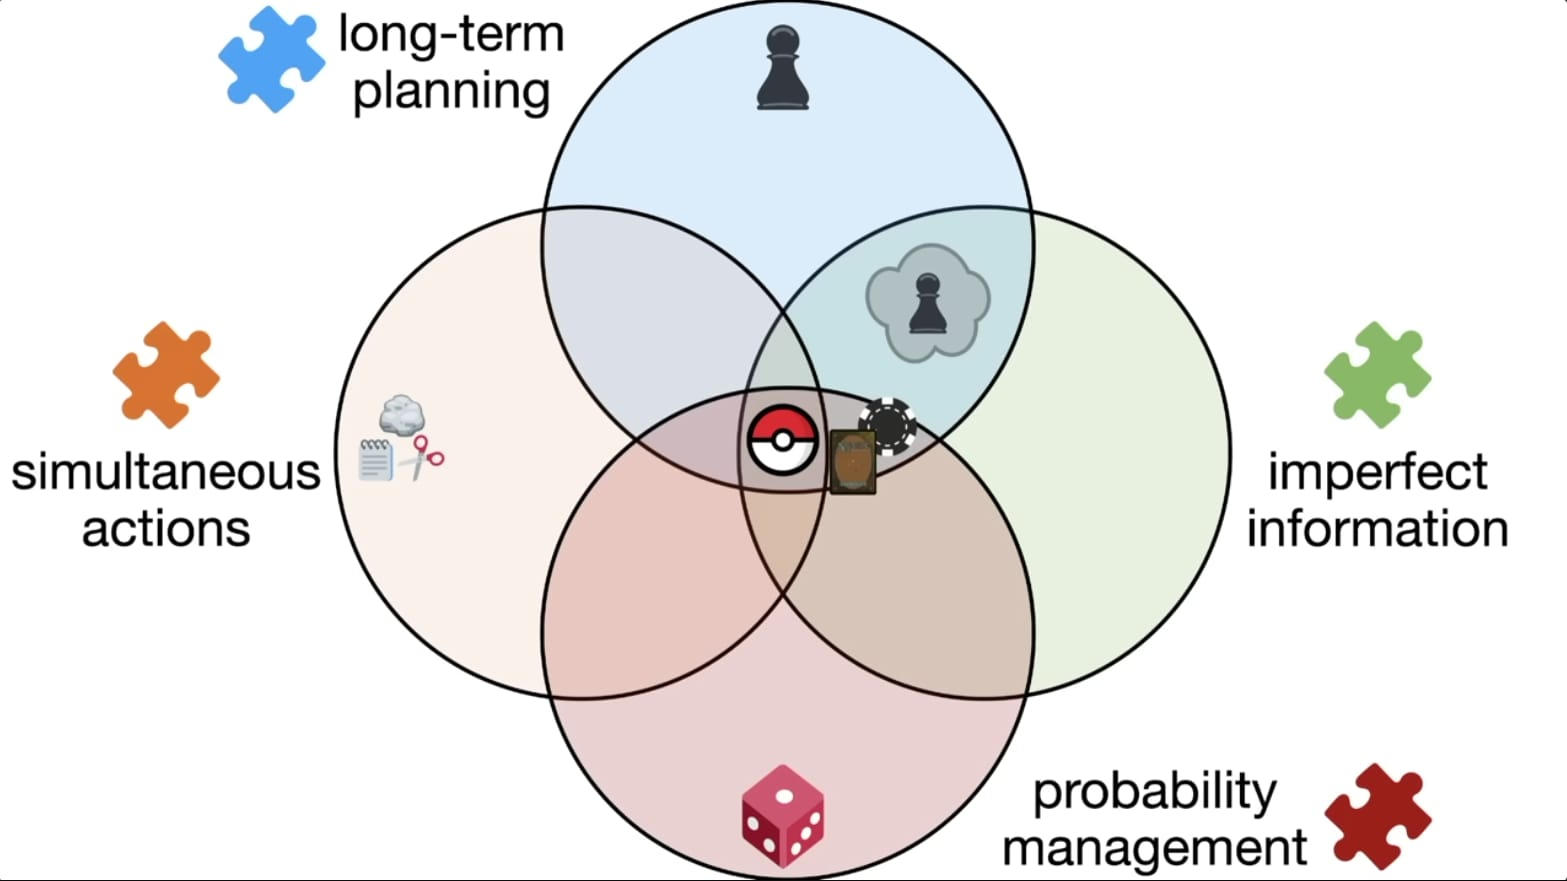
\includegraphics[width=0.75\linewidth]{images/diagrams/stadistical_reason.jpeg}
    \caption{Intersecció dels quatre eixos fonamentals de complexitat en IA i la seva correspondència amb altres jocs.}
    \label{fig:statistical_reason}
\end{figure}

Aquesta combinació única de propietats fa imprescindible formalitzar el problema des de la teoria de jocs i el marc dels processos de decisió sota incertesa. En la secció següent (Secció~\ref{sec:ia_jocs}), es tradueixen aquestes mecàniques al modelat matemàtic rigorós mitjançant Processos de Decisió de Markov Parcialment Observables (POMDP) i Jocs Estocàstics d'Observació Parcial (POSG).

% ============================================================
\section{Formalització matemàtica i marc d'inferència estadística}
\label{sec:ia_jocs}

Una vegada descrites les mecàniques del joc i les seves propietats estructurals (Secció~\ref{sec:pokemon_joc}), aquesta secció formalitza matemàticament el problema des de la teoria de jocs, el marc dels processos de decisió sota incertesa (POMDP i POSG) i estableix les bases d'inferència estadística utilitzades per avaluar rigorosament els agents.

\subsection{De la informació perfecta a la informació imperfecta}

Els jocs han estat el banc de proves clàssic de la IA, des dels escacs~\cite{shannon_chess,CAMPBELL200257} i el Go~\cite{alphago,alphazero} (informació perfecta) fins a videojocs d'estratègia i entorns amb informació amagada com StarCraft~II~\cite{alphastar}, Dota~2~\cite{openai_five} o el pòquer~\cite{libratus,pluribus} (informació imperfecta).

La distinció operativa clau és:
\begin{itemize}
    \item \textbf{Informació perfecta} (escacs, Go): l'estat complet $s$ és comú i totalment visible per a tots els jugadors a cada torn.
    \item \textbf{Informació imperfecta} (pòquer, StarCraft, Pokémon): part de l'estat roman oculta als jugadors. Cal mantenir una distribució de creença sobre les variables no observades i inferir les opcions del rival.
\end{itemize}

\subsection{Formalització dels Processos de Decisió: MDP, POMDP i POSG}

Un \textbf{Procés de Decisió de Markov (MDP)}~\cite{sutton_barto} es defineix com la tupla $(S,A,T,R,\gamma)$, on $S$ és l'espai d'estats, $A$ l'espai d'accions, $T(s'\mid s,a) = P(S_{t+1}=s'\mid S_t=s, A_t=a)$ la funció de transició estocàstica, $R(s,a)$ la funció de recompensa i $\gamma \in [0,1]$ el factor de descompte. La política $\pi(a\mid s)$ maximitza el retorn esperat.

Quan l'agent no observa directament l'estat real $s$, sinó una observació parcial $o\in\Omega$ emesa segons una funció d'emissió $O(o\mid s',a) = P(O_{t+1}=o\mid S_{t+1}=s', A_t=a)$, el model es converteix en un \textbf{Procés de Decisió de Markov Parcialment Observable (POMDP)}~\cite{pomdp,kaelbling_pomdp}.

Atès que a Pokémon hi intervenen dos jugadors que escullen accions de forma simultània sense conèixer la decisió del rival en el torn actual, el model formal conceptualment rigorós és un \textbf{Joc Estocàstic d'Observació Parcial (POSG)}~\cite{shapley_stochastic_games,von_neumann}. Formalsment, un POSG de dos jugadors es defineix com una tupla de vuit components:
\begin{equation}
    \mathcal{M} = \left( N, S, \{A_i\}_{i \in N}, T, \{R_i\}_{i \in N}, \{\Omega_i\}_{i \in N}, \{O_i\}_{i \in N}, \gamma \right)
    \label{eq:posg_tuple}
\end{equation}
on:
\begin{itemize}
    \item $N = \{1, 2\}$ és el conjunt dels dos jugadors (Jugador 1 i Jugador 2).
    \item $S$ és l'espai d'estats globals del joc.
    \item $A_i$ és l'espai d'accions del jugador $i$. Una acció conjunta s'expressa com $\mathbf{a} = (a_1, a_2) \in A_1 \times A_2$.
    \item $T(s'\mid s, \mathbf{a}) = P(S_{t+1}=s'\mid S_t=s, \mathbf{a}_t=\mathbf{a})$ és la probabilitat de transició condicional sota l'acció conjunta.
    \item $R_i(s, \mathbf{a})$ és la recompensa del jugador $i$. En ser un joc competitiu pur de suma zero, es compleix $R_1(s, \mathbf{a}) + R_2(s, \mathbf{a}) = 0$.
    \item $\Omega_i$ és l'espai d'observacions privades del jugador $i$.
    \item $O_i(o_i\mid s', \mathbf{a}) = P(O_{i,t+1}=o_i\mid S_{t+1}=s', \mathbf{a}_t=\mathbf{a})$ és la funció d'emissió d'observacions privades.
    \item $\gamma \in [0, 1]$ és el factor de descompte temporal.
\end{itemize}

\begin{figure}[htbp]
    \centering
    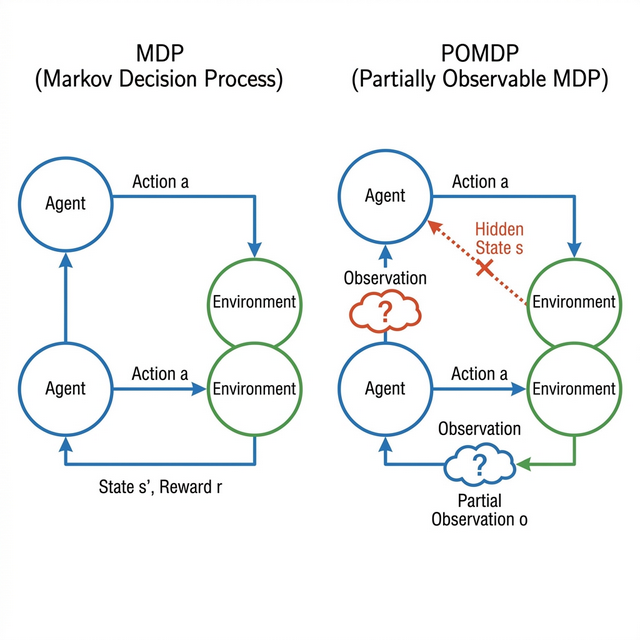
\includegraphics[width=0.72\linewidth]{images/diagrams/mdp_vs_pomdp.png}
    \caption{Diferència conceptual entre un MDP, un POMDP i un POSG. En el POMDP l'agent rep una observació parcial de l'estat. Una batalla Pokémon afegeix un segon decisor simultani i s'aproxima exactament amb un POSG.}
    \label{fig:mdp_pomdp}
\end{figure}

\subsection{Estat de creença, matriu de pagaments i reducció d'enginyeria}

A causa de la informació oculta, el jugador $i$ no pot basar la seva decisió directament en l'estat real $s$, sinó en un \textbf{estat de creença} (\emph{Belief State}) $b_{i,t}(s) \in \Delta(S)$, definit com la distribució de probabilitat sobre els possibles estats globals $s$ donada la seva història d'observacions i accions $h_{i,t} = (o_{i,1}, a_{i,1}, \dots, o_{i,t})$:
\begin{equation}
    b_{i,t}(s) = P(S_t = s \mid h_{i,t})
    \label{eq:belief_state}
\end{equation}
Aquest estat de creença s'actualitza a cada torn mitjançant la regla de Bayes al rebre la nova observació $o_{i,t+1}$.

D'altra banda, a causa de la simultaneïtat de les accions, a cada pas de decisió els dos jugadors s'enfronten a una matriu de pagaments de forma normal $M(a_1, a_2) = \mathbb{E}_{s \sim b} [R_1(s, a_1, a_2) + \gamma V(s')]$. Com que qualsevol política pura determinista $\pi_i(a_i)$ és explotable per l'oponent (p. ex., si un agent ataca de manera predictible, el rival canviarà a un Pokémon immune), les polítiques òptimes requereixen la selecció de \textbf{polítiques estocàstiques / estratègies mixtes} $\pi_1 \in \Delta(A_1)$ i $\pi_2 \in \Delta(A_2)$ per assolir un \textbf{Equilibri de Nash}:
\begin{equation}
    \mathbb{E}_{\mathbf{a} \sim (\pi_1^*, \pi_2^*)} [R_1(s, \mathbf{a})] \ge \mathbb{E}_{a_1 \sim \pi_1, a_2 \sim \pi_2^*} [R_1(s, a_1, a_2)], \qquad \forall \pi_1 \in \Delta(A_1)
    \label{eq:nash_equilibrium}
\end{equation}

Des del punt de vista computacional, resoldre un POSG general és un problema de complexitat $NEXP$-hard. Per aquest motiu, els cinc paradigmes desenvolupats en aquest treball apliquen reduccions d'enginyeria:
\begin{itemize}
    \item \textbf{Aprenentatge per Reforç (PPO) i Clonatge Conductual (XGBoost)}: Absorbeixen la política del rival $\pi_2(a_2 \mid o_2)$ dins de la funció de transició de l'entorn:
          \begin{equation}
              T_{\mathrm{eff}}(s'\mid s, a_1) = \sum_{a_2 \in A_2} \pi_2(a_2 \mid o_2) \cdot T(s'\mid s, a_1, a_2)
              \label{eq:eff_transition}
          \end{equation}
          Aquesta reducció transforma el POSG multijugador en un \textbf{POMDP de decisió individual} des de la perspectiva de l'agent.
    \item \textbf{Cerca Minimax i MCTS}: Construeixen localment la matriu de respostes o simulen *rollouts* d'esperança sobre l'arbre de decisions d'un torn o de pocs torns a l'arrel.
\end{itemize}

\subsection{Instanciació dels components a \texttt{gen9randombattle}}

A la Taula~\ref{tab:pomdp_pokemon} es detalla com es mapeja exactament cadascun dels components formals del POSG/POMDP al domini del combat individual de \texttt{gen9randombattle}.

\begin{table}[H]
    \centering
    \small
    \begin{tabular}{|l|p{10.5cm}|}
        \hline
        \textbf{Component} & \textbf{Instanciació a Singles \texttt{gen9randombattle}}                                                                                                                                    \\ \hline
        $S$                & Sis Pokémon per bàndol (espècie, HP, configuració, objecte, habilitat, modificadors i condició d'estat), clima, perills d'entrada, Tera consumit i torn. $|S|$ és astronòmic i no s'enumera. \\ \hline
        $A$                & Fins a quatre moviments, cinc canvis i la Teracristal·lització com a modificador. La legalitat depèn de PP, debilitaments i bloqueigs; el PPO ho codifica en 14 índexs.                      \\ \hline
        $T$                & Motor de Showdown: dany amb roll $[0{,}85,1{,}00]$, STAB, Taula de Tipus, prioritat, velocitat, secundaris.                                                                                  \\ \hline
        $R$                & Recompensa terminal conceptual $+1$ per victòria i $-1$ per derrota. Per a l'avaluació s'enregistra l'indicador binari $W\in\{0,1\}$ i se'n publica la mitjana.                              \\ \hline
        $\Omega$           & Equip propi complet; del rival, espècies revelades, percentatge d'HP, moviments utilitzats i condicions laterals. EV, naturalesa, objecte i moviments no revelats romanen ocults.            \\ \hline
    \end{tabular}
    \caption{Mapatge POSG/POMDP al combat individual de Random Battle (Generació~IX).}
    \label{tab:pomdp_pokemon}
\end{table}

\subsection{Marc d'avaluació estadística i mètodes d'inferència}
\label{subsec:marc_estadistic}

Per comparar de manera científicament rigorosa la capacitat de decisió dels 28 agents desenvolupats, s'estableix un marc d'inferència estadística basat en tres eines fonamentals:

\begin{enumerate}
    \item \textbf{Estimació de la Taxa de Victòria (\emph{Win Rate}):}
          En un enfrontament de $N$ partides entre dos agents, cada combat $i$ s'escriu com una variable aleatòria binària de Bernoulli $W_i \sim \mathrm{Bernoulli}(p)$, on $W_i = 1$ indica victòria de l'agent i $W_i = 0$ indica derrota. L'estimador puntual de la taxa de victòria $\hat{p}$ és la mitjana mostral:
          \begin{equation}
              \hat{p} = \frac{1}{N} \sum_{i=1}^N W_i
              \label{eq:win_rate_estimator}
          \end{equation}

    \item \textbf{Intervals de Confiança de Wilson (\emph{Wilson Score Interval}):}
          A diferència de l'interval binomi estàndard de Wald ($\hat{p} \pm z \sqrt{\hat{p}(1-\hat{p})/N}$), que falla prop dels límits ($0$ o $1$) o en mostres asimètriques, aquest treball calcula els intervals de confiança mitjançant l'\textbf{interval de la puntuació de Wilson}~\cite{wilson_1927}:
          \begin{equation}
              \mathrm{CI}_{\mathrm{Wilson}} = \frac{1}{1 + \frac{z^2}{N}} \left( \hat{p} + \frac{z^2}{2N} \pm z \sqrt{\frac{\hat{p}(1-\hat{p})}{N} + \frac{z^2}{4N^2}} \right)
              \label{eq:wilson_ci}
          \end{equation}
          on $z = z_{1-\alpha/2} = 1{,}96$ per a un nivell de confiança del $95\%$ ($\alpha = 0{,}05$).

    \item \textbf{Sistema de Puntuació Elo i Model de Bradley-Terry:}
          Per ordenar els 28 agents en un llistat global independent de parelles individuals, s'utilitza el model de comparació per parelles de Bradley-Terry / Sistema de Puntuació Elo~\cite{elo_rating,bradley_terry_1952}. La probabilitat esperada de victòria de l'agent $A$ enfront de l'agent $B$ amb puntuacions $R_A$ i $R_B$ ve donada per la funció logística:
          \begin{equation}
              E_A = \frac{1}{1 + 10^{(R_B - R_A)/400}}
              \label{eq:elo_expected}
          \end{equation}
          I l'actualització de la puntuació Elo després de cada combat amb resultat $S_A \in \{0, 1\}$ segueix:
          \begin{equation}
              R_A' = R_A + K (S_A - E_A)
              \label{eq:elo_update}
          \end{equation}
          on $K$ és el factor d'ajust d'escala.
\end{enumerate}

Finalment, la reducció de la variància de generació d'equips s'aconsegueix mitjançant un volum massiu d'avaluació ($N > 6{,}4 \times 10^6$ batalles totals), la qual cosa redueix l'error estàndard $SE = \sqrt{\frac{p(1-p)}{N}}$ per sota del $0{,}3\%$ ($SE < 0{,}003$), danyant una significança estadística del $p < 0{,}001$ en totes les comparacions presentades als Capítols~\ref{chap:metodologia} i~\ref{chap:resultats}.

% ============================================================
\section{Estat de l'Art en IA i Pokémon}
\label{sec:estat_art}

\textit{poke-env}~\cite{poke_env,pokemon_ai_sahovic} va facilitar l'ús de Pokémon Showdown com a entorn d'aprenentatge. La biblioteca inclou \texttt{RandomPlayer}, \texttt{MaxBasePowerPlayer} i \texttt{SimpleHeuristicsPlayer}.

Huang i Lee~\cite{pokemon_rl_huang} van entrenar un agent PPO amb \textit{self-play} a Showdown. Més recentment, Grigsby et al.~\cite{grigsby_metamon} van aplicar imitació i RL fora de línia amb Transformers (*Metamon*) sobre repeticions humanes. \textit{PokéChamp}~\cite{pokechamp,pokechamp_icml} combina un model de llenguatge (LLM) amb cerca minimax d'un pas i va assolir el Top 3 d'Elo al ladder públic de Showdown. \textit{PokéLLMon}~\cite{pokellmon} utilitza així mateix models de llenguatge per a la presa de decisions en combat.

\subsection{Què afegeix aquest TFM}

\begin{enumerate}
    \item \textbf{Una matriu comuna de 28 agents} per a heurístiques, minimax, MCTS ras i imitació, amb oponents compartits, volums mostrals explícits ($>6{,}4$M de batalles) i telemetria per decisió.
    \item \textbf{Una seqüència de catorze heurístiques} (\texttt{v1}--\texttt{v14}) que permet estudiar ablacions de coneixement de domini.
    \item \textbf{Variants guiades i no guiades} de cerca i d'imitació, amb \texttt{v14} com a prior o executor.
    \item \textbf{Una avaluació rigorosa de MaskablePPO} contra \texttt{v12}, amb inicialització per clonatge conductual.
\end{enumerate}

% ============================================================
\section{Fonaments teòrics dels cinc paradigmes de decisió}
\label{sec:ia_tecniques}

Cada paradigma introdueix un mecanisme diferent: coneixement codificat, anticipació adversària, simulació, supervisió amb dades humanes o optimització per reforç.

\begin{table}[htbp]
\centering
\caption{Comparació conceptual dels cinc paradigmes. Tots decideixen sobre el mateix simulador i format; canvia la font de coneixement i el còmput per torn.}
\label{tab:paradigm_mechanisms}
\small
\renewcommand{\arraystretch}{1.3}
\begin{tabularx}{\textwidth}{l>{\raggedright\arraybackslash}X>{\raggedright\arraybackslash}X>{\raggedright\arraybackslash}X>{\raggedright\arraybackslash}p{2.2cm}}
\toprule
\textbf{Paradigma} & \textbf{Què decideix} & \textbf{Coneixement} & \textbf{Còmput per torn} & \textbf{Aprèn?} \\
\midrule
Heurística & Argmax d'una puntuació fixa sobre accions legals. & Regles escrites (dany, posició, Tera). & Constant, baix. & No durant l'execució. \\
\arrayrulecolor{gray!30}\hline\arrayrulecolor{black}
Minimax d'un torn & Maximin sobre una matriu d'accions i respostes estimades. & Funció de fulla + prior opcional. & Enumeració d'un torn. & No. \\
\arrayrulecolor{gray!30}\hline\arrayrulecolor{black}
MCTS ras & UCB/PUCT només als fills de l'arrel. & Determinització i, a \texttt{v20}, prior de \texttt{v14}. & 100 simulacions de 5 torns. & No (cerca en línia). \\
\arrayrulecolor{gray!30}\hline\arrayrulecolor{black}
Imitació & Classificador atacar/canviar + executor. & Trajectòries humanes Elo~$1800+$. & Inferència XGBoost. & Supervisat, fora de línia. \\
\arrayrulecolor{gray!30}\hline\arrayrulecolor{black}
PPO & Política estocàstica emmascarada $\pi_\theta(a\mid o)$. & Interacció amb recompensa + clonatge inicial. & Un pas de xarxa. & Per reforç, fora de partida. \\
\bottomrule
\end{tabularx}
\end{table}


\subsection{Heurístiques: coneixement com a ablació}

Una heurística no ajusta els seus paràmetres durant l'execució. A cada decisió puntua les accions legals amb regles fixes i tria l'argmax. La seqüència \texttt{v1}--\texttt{v14} funciona com una \textbf{ablació incremental}: permet relacionar blocs de coneixement amb canvis de rendiment.

\subsection{Minimax d'un torn: resposta adversària immediata}

Minimax~\cite{minimax_knuth} assigna a cada estat el valor de la millor acció sota la resposta més desfavorable. Com que a Pokémon les accions del torn són simultànies, la implementació construeix una matriu d'accions pròpies i respostes rivals estimades (\texttt{v15}--\texttt{v17}). La funció de fulla de \texttt{v15} és:
\begin{equation}
    V = \mathrm{HP}_{\mathrm{me}} - 1{,}5\,\mathrm{HP}_{\mathrm{opp}} + \text{bonificacions}.
\end{equation}
\texttt{v16} afegeix bonificacions posicionals i \texttt{v17} suma un prior de $+0{,}15$ a l'acció de \texttt{v14}.

\subsection{Cerca de Monte Carlo a l'arrel (shallow MCTS)}

L'MCTS complet~\cite{mcts_survey,coulom_mcts} alterna selecció, expansió, simulació i retropropagació en un arbre. La implementació d'aquest treball (\texttt{v18}--\texttt{v20}) aplica UCB1 o PUCT només als fills de l'\textbf{arrel}, executant 100 simulacions de 5 torns amb \texttt{LocalSim}~\cite{pokechamp}.

\begin{figure}[htbp]
    \centering
    \begin{tikzpicture}[
            font=\small,
            box/.style={rectangle, rounded corners, draw, align=center, minimum height=1.05cm, text width=2.55cm},
            arr/.style={->, thick, >=stealth}
        ]
        \node[box, fill=blue!12] (sel) {\textbf{1. Selecció}\\UCB / PUCT};
        \node[box, fill=green!12, right=0.45cm of sel] (exp) {\textbf{2. Expansió}\\nou fill};
        \node[box, fill=orange!12, right=0.45cm of exp] (sim) {\textbf{3. Simulació}\\rollout};
        \node[box, fill=purple!12, right=0.45cm of sim] (back) {\textbf{4. Còpia enrere}\\actualitza $Q,n$};
        \draw[arr] (sel) -- (exp);
        \draw[arr] (exp) -- (sim);
        \draw[arr] (sim) -- (back);
        \draw[arr] (back.south) -- ++(0,-0.45) -| node[below, font=\scriptsize, pos=0.25] {aquest TFM: només fills de l'arrel} (sel.south);
    \end{tikzpicture}
    \caption{Cicle clàssic de l'MCTS adaptat a simulacions de 5 torns a l'arrel.}
    \label{fig:mcts_cycle}
\end{figure}

UCB1:
\begin{equation}
    \mathrm{UCB1}(j) = \bar X_j + C\sqrt{\frac{\ln N}{n_j}}, \qquad C=1{,}4.
\end{equation}
PUCT (\texttt{v20}) afegeix un prior $\pi(a)$ extret de \texttt{v14} amb un pes de $0{,}70$.

\subsection{Imitació / clonatge conductual}

L'aprenentatge per imitació (\textit{behavioral cloning}) premia imitar trajectòries d'experts~\cite{pomerleau_alvinn,argall_lfd}. \texttt{v21} utilitza un model XGBoost~\cite{xgboost} sobre 1,12 milions de torns d'experts (Elo~$1800+$) per a la decisió macro i delega a \texttt{v14} l'execució micro. \texttt{v22} és un model dual purament d'imitació (dos classificadors XGBoost).

\subsection{PPO amb emmascarament d'accions}

L'aprenentatge per reforç~\cite{sutton_barto} optimitza una política d'actor-crític~\cite{konda_actor_critic}. MaskablePPO~\cite{ppo,huang_action_masking,sb3_contrib} utilitza l'objectiu retallat:
\begin{equation}
    L^{\mathrm{CLIP}}(\theta)=\hat{\mathbb{E}}_t\left[\min\left(r_t(\theta)\hat A_t,\;\mathrm{clip}(r_t(\theta),1-\epsilon,1+\epsilon)\hat A_t\right)\right].
\end{equation}

\begin{figure}[htbp]
    \centering
    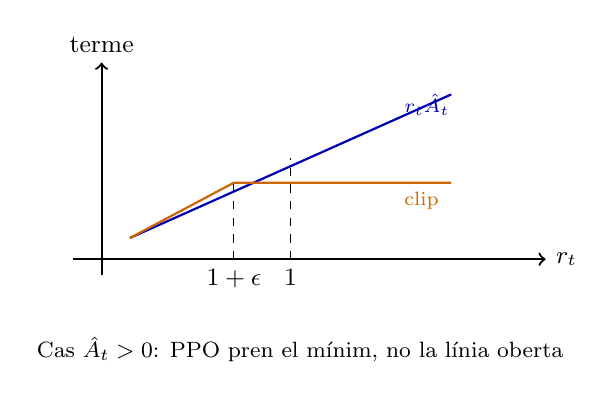
\begin{tikzpicture}[font=\small, x=2.4cm, y=1.35cm]
        \draw[->, thick] (-0.15,0) -- (2.35,0) node[right] {$r_t$};
        \draw[->, thick] (0,-0.15) -- (0,1.85) node[above] {terme};
        \draw[thick, blue!70!black] (0.15,0.2) -- (1.85,1.55);
        \draw[thick, orange!80!black] (0.15,0.2) -- (0.7,0.72) -- (1.85,0.72);
        \draw[dashed] (0.7,0) node[below] {$1+\epsilon$} -- (0.7,0.72);
        \draw[dashed] (1,0) node[below] {$1$} -- (1,0.95);
        \node[font=\scriptsize, blue!70!black, anchor=west] at (1.55,1.45) {$r_t\hat A_t$};
        \node[font=\scriptsize, orange!80!black, anchor=west] at (1.55,0.55) {clip};
        \node[font=\footnotesize] at (1.05,-0.85) {Cas $\hat A_t>0$: PPO pren el mínim, no la línia oberta};
    \end{tikzpicture}
    \caption{Intuïció de l'objectiu retallat de PPO.}
    \label{fig:ppo_clip}
\end{figure}

L'emmascarament d'accions assigna probabilitat nul·la a accions il·legals. El clonatge conductual previ inicialitza l'actor a partir de 400 partides de \texttt{v8}.

% ============================================================
\section{Síntesi del marc teòric}
\label{sec:marc_teoric_sintesi}

El marc teòric queda definit per les mecàniques del combat Pokémon individual, el format \texttt{gen9randombattle}, la formalització matemàtica POSG/POMDP i els fonaments dels cinc paradigmes d'agents. Aquestes bases permeten avaluar amb rigor experimental els resultats empírics que es presenten als capítols següents.
